\documentclass[]{beamer}
\usetheme[block=fill,progressbar=frametitle,numbering=none]{metropolis}
% Paquetes de la ams
\usepackage{amsmath,amsthm,amssymb,amsfonts}
% Codificacion UTF-8
\usepackage[utf8]{inputenc}
% Tablas e imagenes en espaniol
\usepackage[spanish,es-tabla]{babel}
% Mejores graficos
\usepackage{graphicx}
% tablas mas lindas
\usepackage{booktabs}
% Links a urls
\usepackage{url}
% Linkear referencias en pdfs
\usepackage{hyperref}
% Texto mas lindo para los pie de figura
\usepackage[margin=10pt,font=small,labelfont=bf, labelsep=endash]{caption}

% Citas
\usepackage[backend=biber,style=ieee]{biblatex}
\addbibresource{biblio.bib}

% Codigo
\usepackage{listings}

% Dir tree
\usepackage{dirtree}

% Pagina en blanco cuando ha
\usepackage{emptypage}

\definecolor{A11}{HTML}{B2DF8A}
\definecolor{A12}{HTML}{33A02C}
\definecolor{A23}{HTML}{FDBF6F}
\definecolor{A24}{HTML}{FF7F00}
\definecolor{B15}{HTML}{FB9A99}
\definecolor{B16}{HTML}{E31A1C}
\definecolor{B27}{HTML}{A6CEE3}
\definecolor{B28}{HTML}{1F78B4}

% Ejemplos, observaciones y teorema
\theoremstyle{definition}
\newtheorem{exa}{Ejemplo}[section]
\newtheorem*{obs}{Observación}
\newtheorem{que}{Pregunta}[section]
\newtheorem{dex}{Definicion}[section]

\author{Francisco Nemiña}
\title{Nivel 2: herramientas de teledetección cuantitativa}
\subtitle{El espectro electromagnético}
\institute{Unidad de Educación y Formación Masiva \\ Comisión Nacional de Actividades Espaciales}
\date{}
\graphicspath{{./figs/}}

\begin{document}

\maketitle

\begin{frame}{Table of contents}
  \setbeamertemplate{section in toc}[sections numbered]
  \tableofcontents[hideallsubsections]
\end{frame}
\begin{frame}{Firma espectral}
  Si ahora pensamos como depende la reflectancia de la longitud de onda podemos definir
  \begin{block}{Definición}
    Llamamos firma espectral a la función de la reflectancia como función de la longitud de onda, $\rho_\lambda$.
  \end{block}\pause
  Veamos algunos ejemplos y de por que sirven para describir a las coberturas.\pause
  \begin{itemize}
    \item Vegetación
    \item Suelo
    \item Agua
  \end{itemize}
\end{frame}


\begin{frame}{Firma espectral - vegetación}
  \begin{figure}
  \
  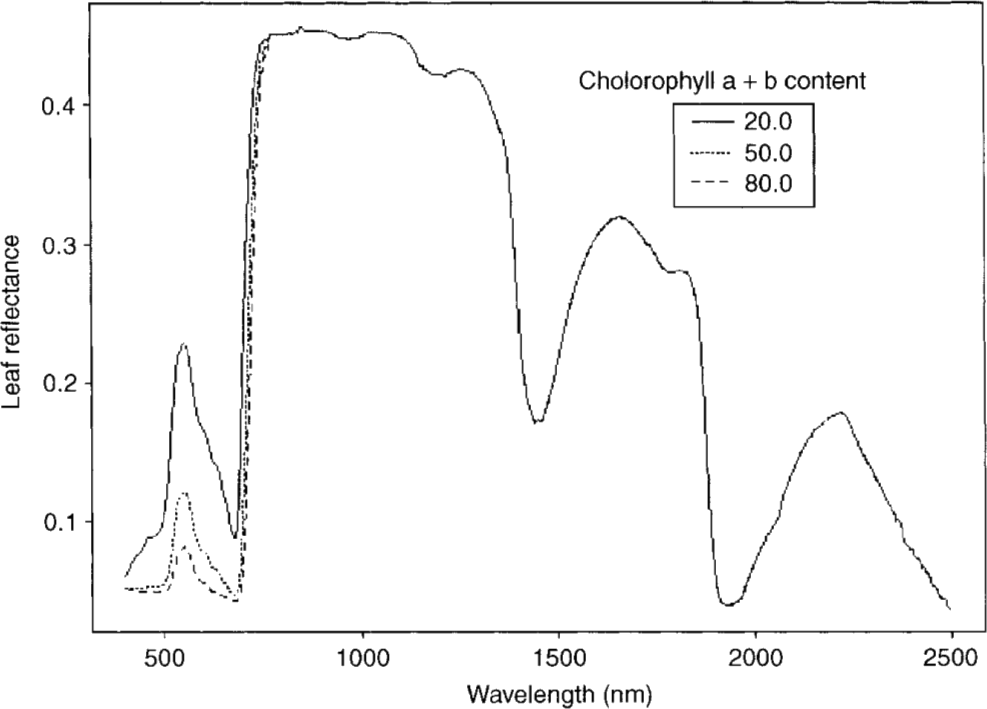
\includegraphics[width=0.8\textwidth]{clorovar.png}
  \caption{Variaciones de la firma espectral con el contenido de clorofila.\footfullcite{liang2005quantitative}}
  \end{figure}
\end{frame}
%--- Next Frame ---%

\begin{frame}{Firma espectral - vegetación}
  \begin{figure}

  \includegraphics[width=0.8\textwidth]{vwvar.png}
  \caption{Variaciones de la firma espectral con el contenido de agua.\footfullcite{liang2005quantitative}}
  \end{figure}
\end{frame}
%--- Next Frame ---%

\begin{frame}{Firma espectral - vegetación}
  \begin{figure}

  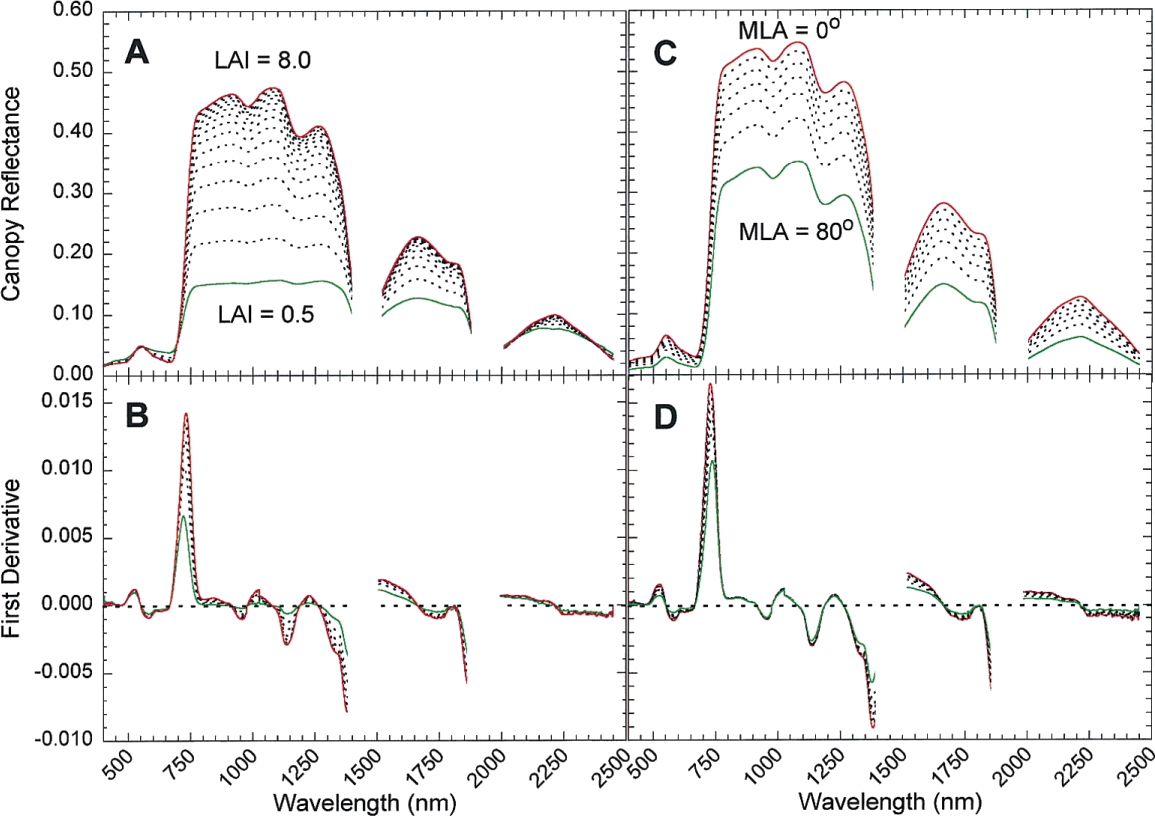
\includegraphics[width=0.8\textwidth]{leafvar.png}
  \caption{Variaciones de la firma espectral con el área foliar.\footfullcite{asner1998biophysical}}
  \end{figure}
\end{frame}
%--- Next Frame ---%

\begin{frame}{Firma espectral - vegetación}
    \begin{figure}

    \includegraphics[width=0.8\textwidth]{vivomuerto.png}
    \caption{Firma espectral de la vegetación en diferentes estados.\footfullcite{asner1998biophysical}}
    \end{figure}
\end{frame}
%--- Next Frame ---%

\begin{frame}{Firma espectral - suelo}
    \begin{figure}

    \includegraphics[width=0.6\textwidth]{soilvar.png}
    \caption{Firma espectral del suelo con distintos contenidos de humedad.\footfullcite{liang2005quantitative}}
    \end{figure}
\end{frame}
%--- Next Frame ---%

\begin{frame}{Firma espectral - agua}
    \begin{figure}

    \includegraphics[width=0.8\textwidth]{waterm.png}
    \caption{Firma espectral de agua con distinto contenido de arcilla disuelta.\footfullcite{clark2007usgs}}
    \end{figure}
\end{frame}
%--- Next Frame ---%

\begin{frame}{Firma espectral - agua}
    \begin{figure}
    \includegraphics[width=0.8\textwidth]{snow.png}
    \caption{Firma espectral de agua en distintos estados de agregación.\footfullcite{snow}}
    \end{figure}
\end{frame}
%--- Next Frame ---%

\end{document}
